\begin{figure}
        \centering
        \begin{subfigure}[b]{0.5\textwidth}
                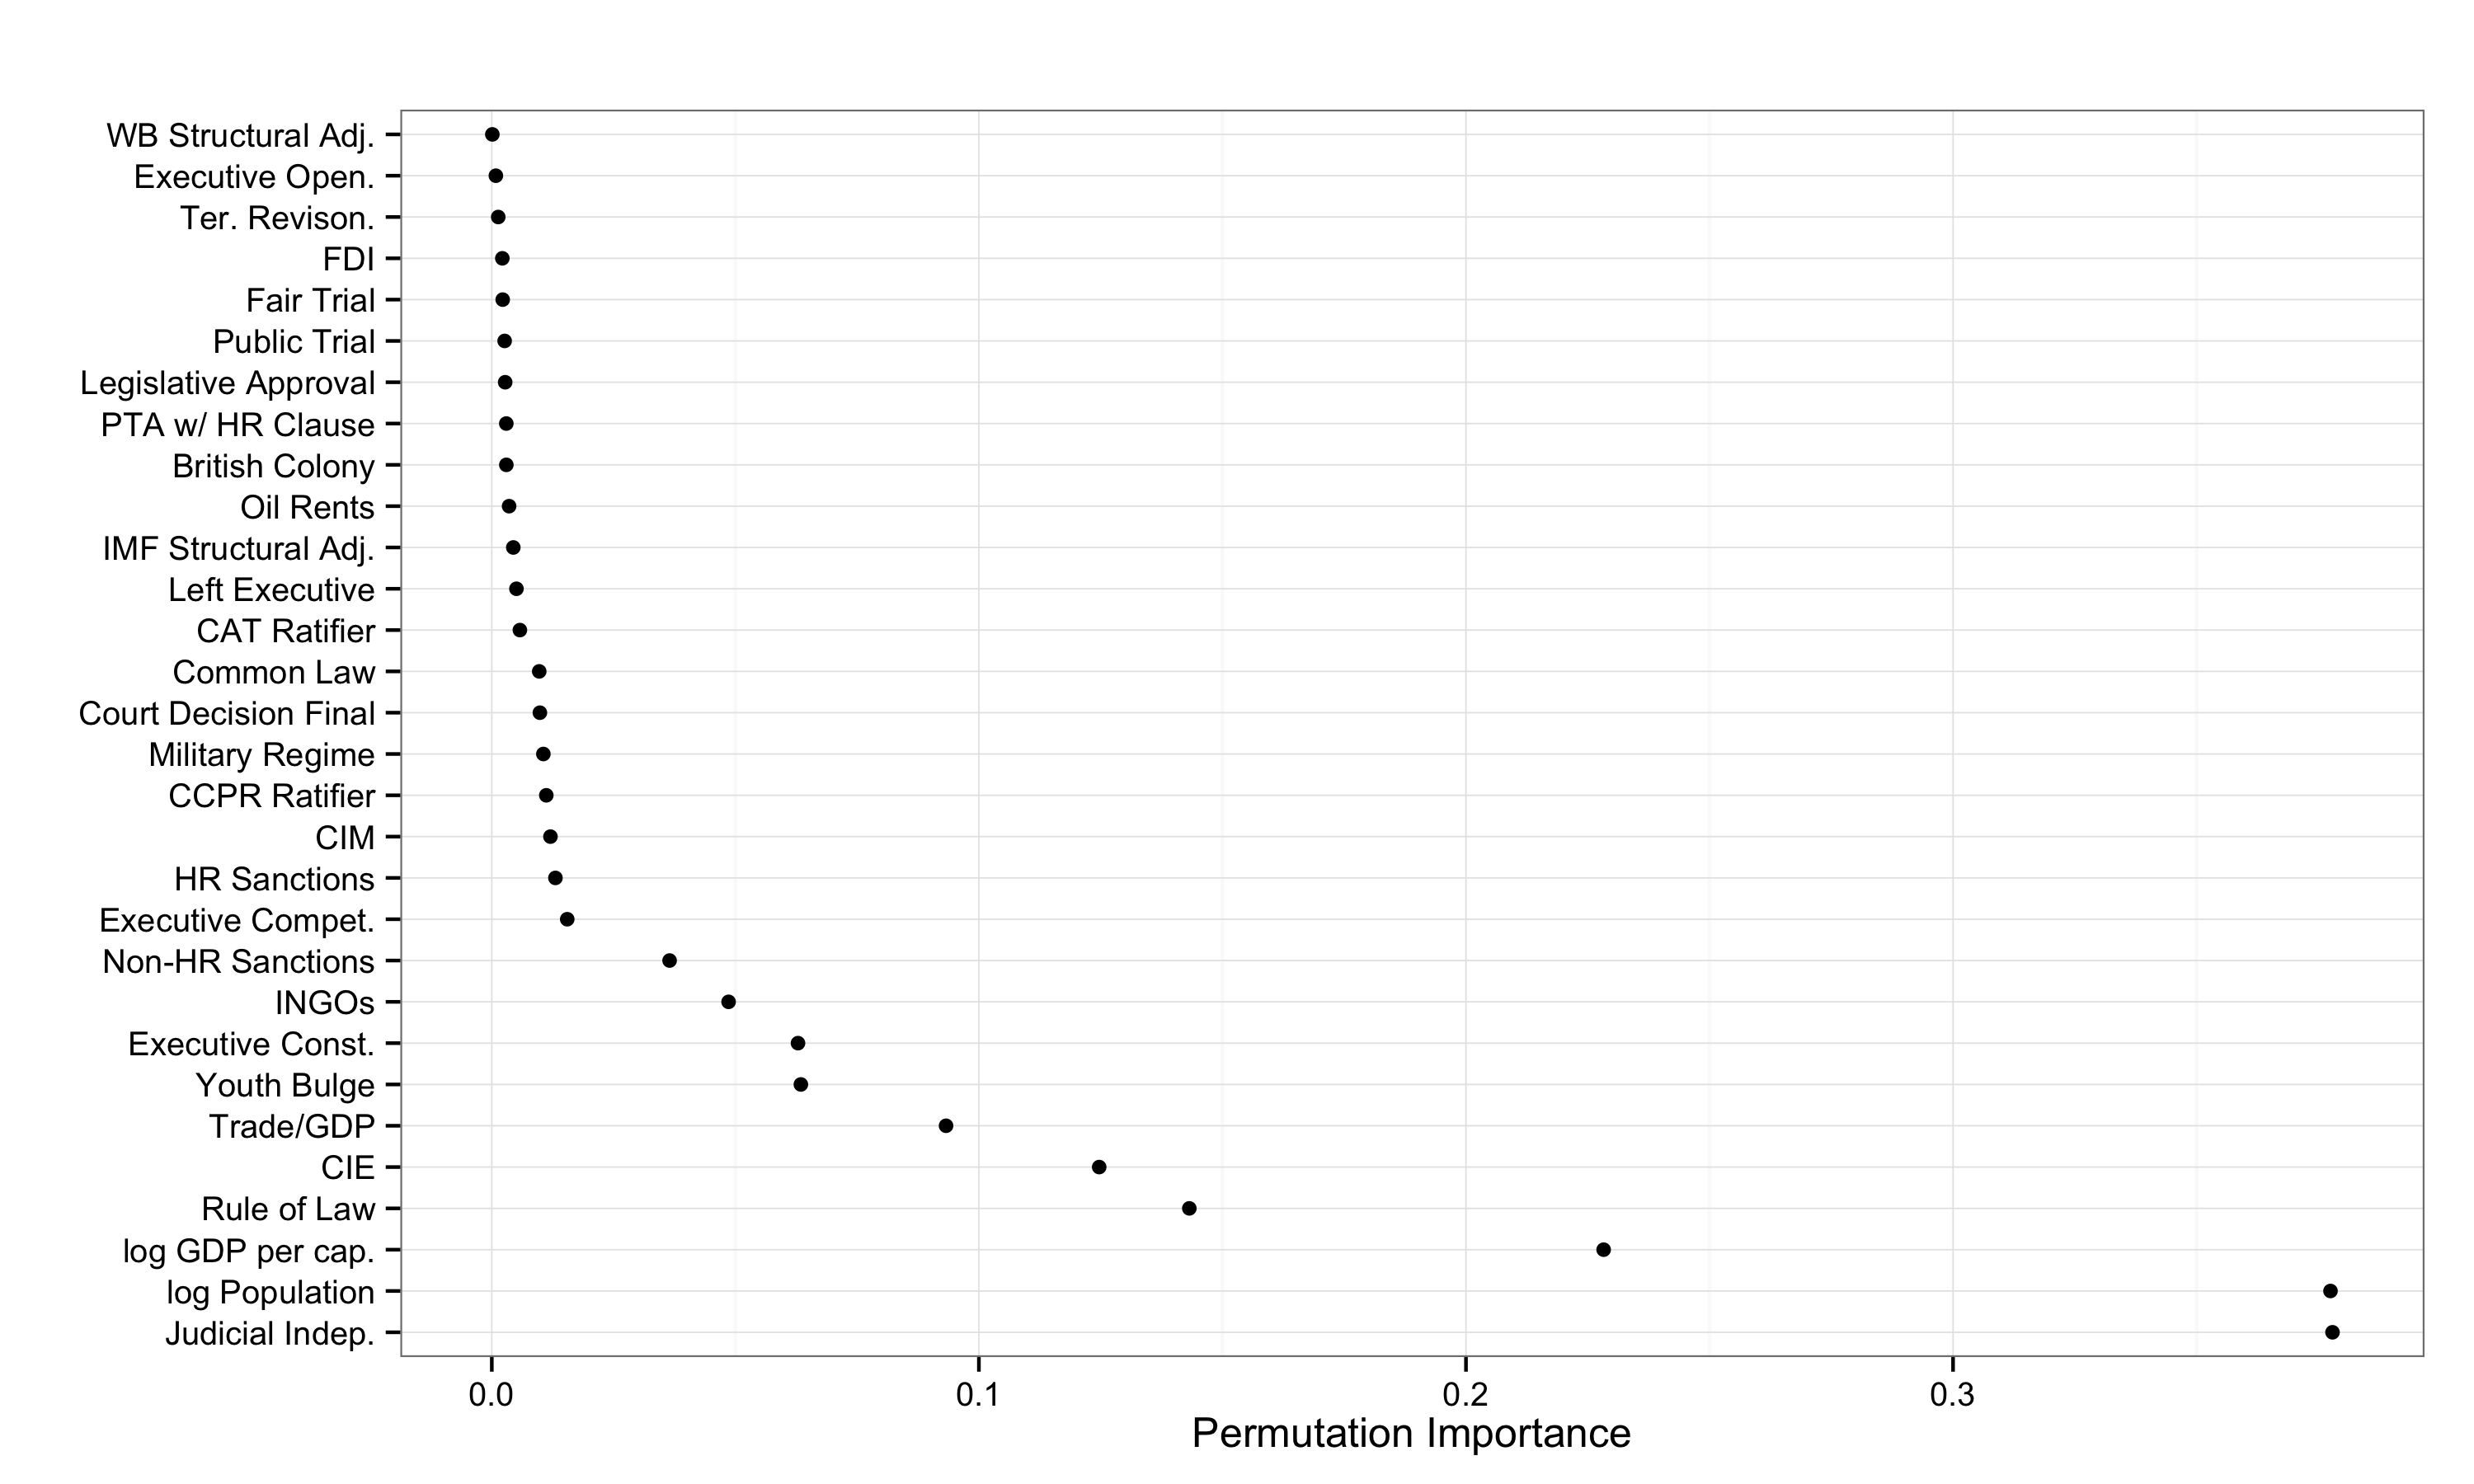
\includegraphics[width=\textwidth]{figures/latent_imp.png}
                \caption{Permutation importance for human rights data.}
                \label{fig:latent_imp}
        \end{subfigure}%
        ~ %add desired spacing between images, e. g. ~, \quad, \qquad, \hfill etc.
          %(or a blank line to force the subfigure onto a new line)
        \begin{subfigure}[b]{0.5\textwidth}
                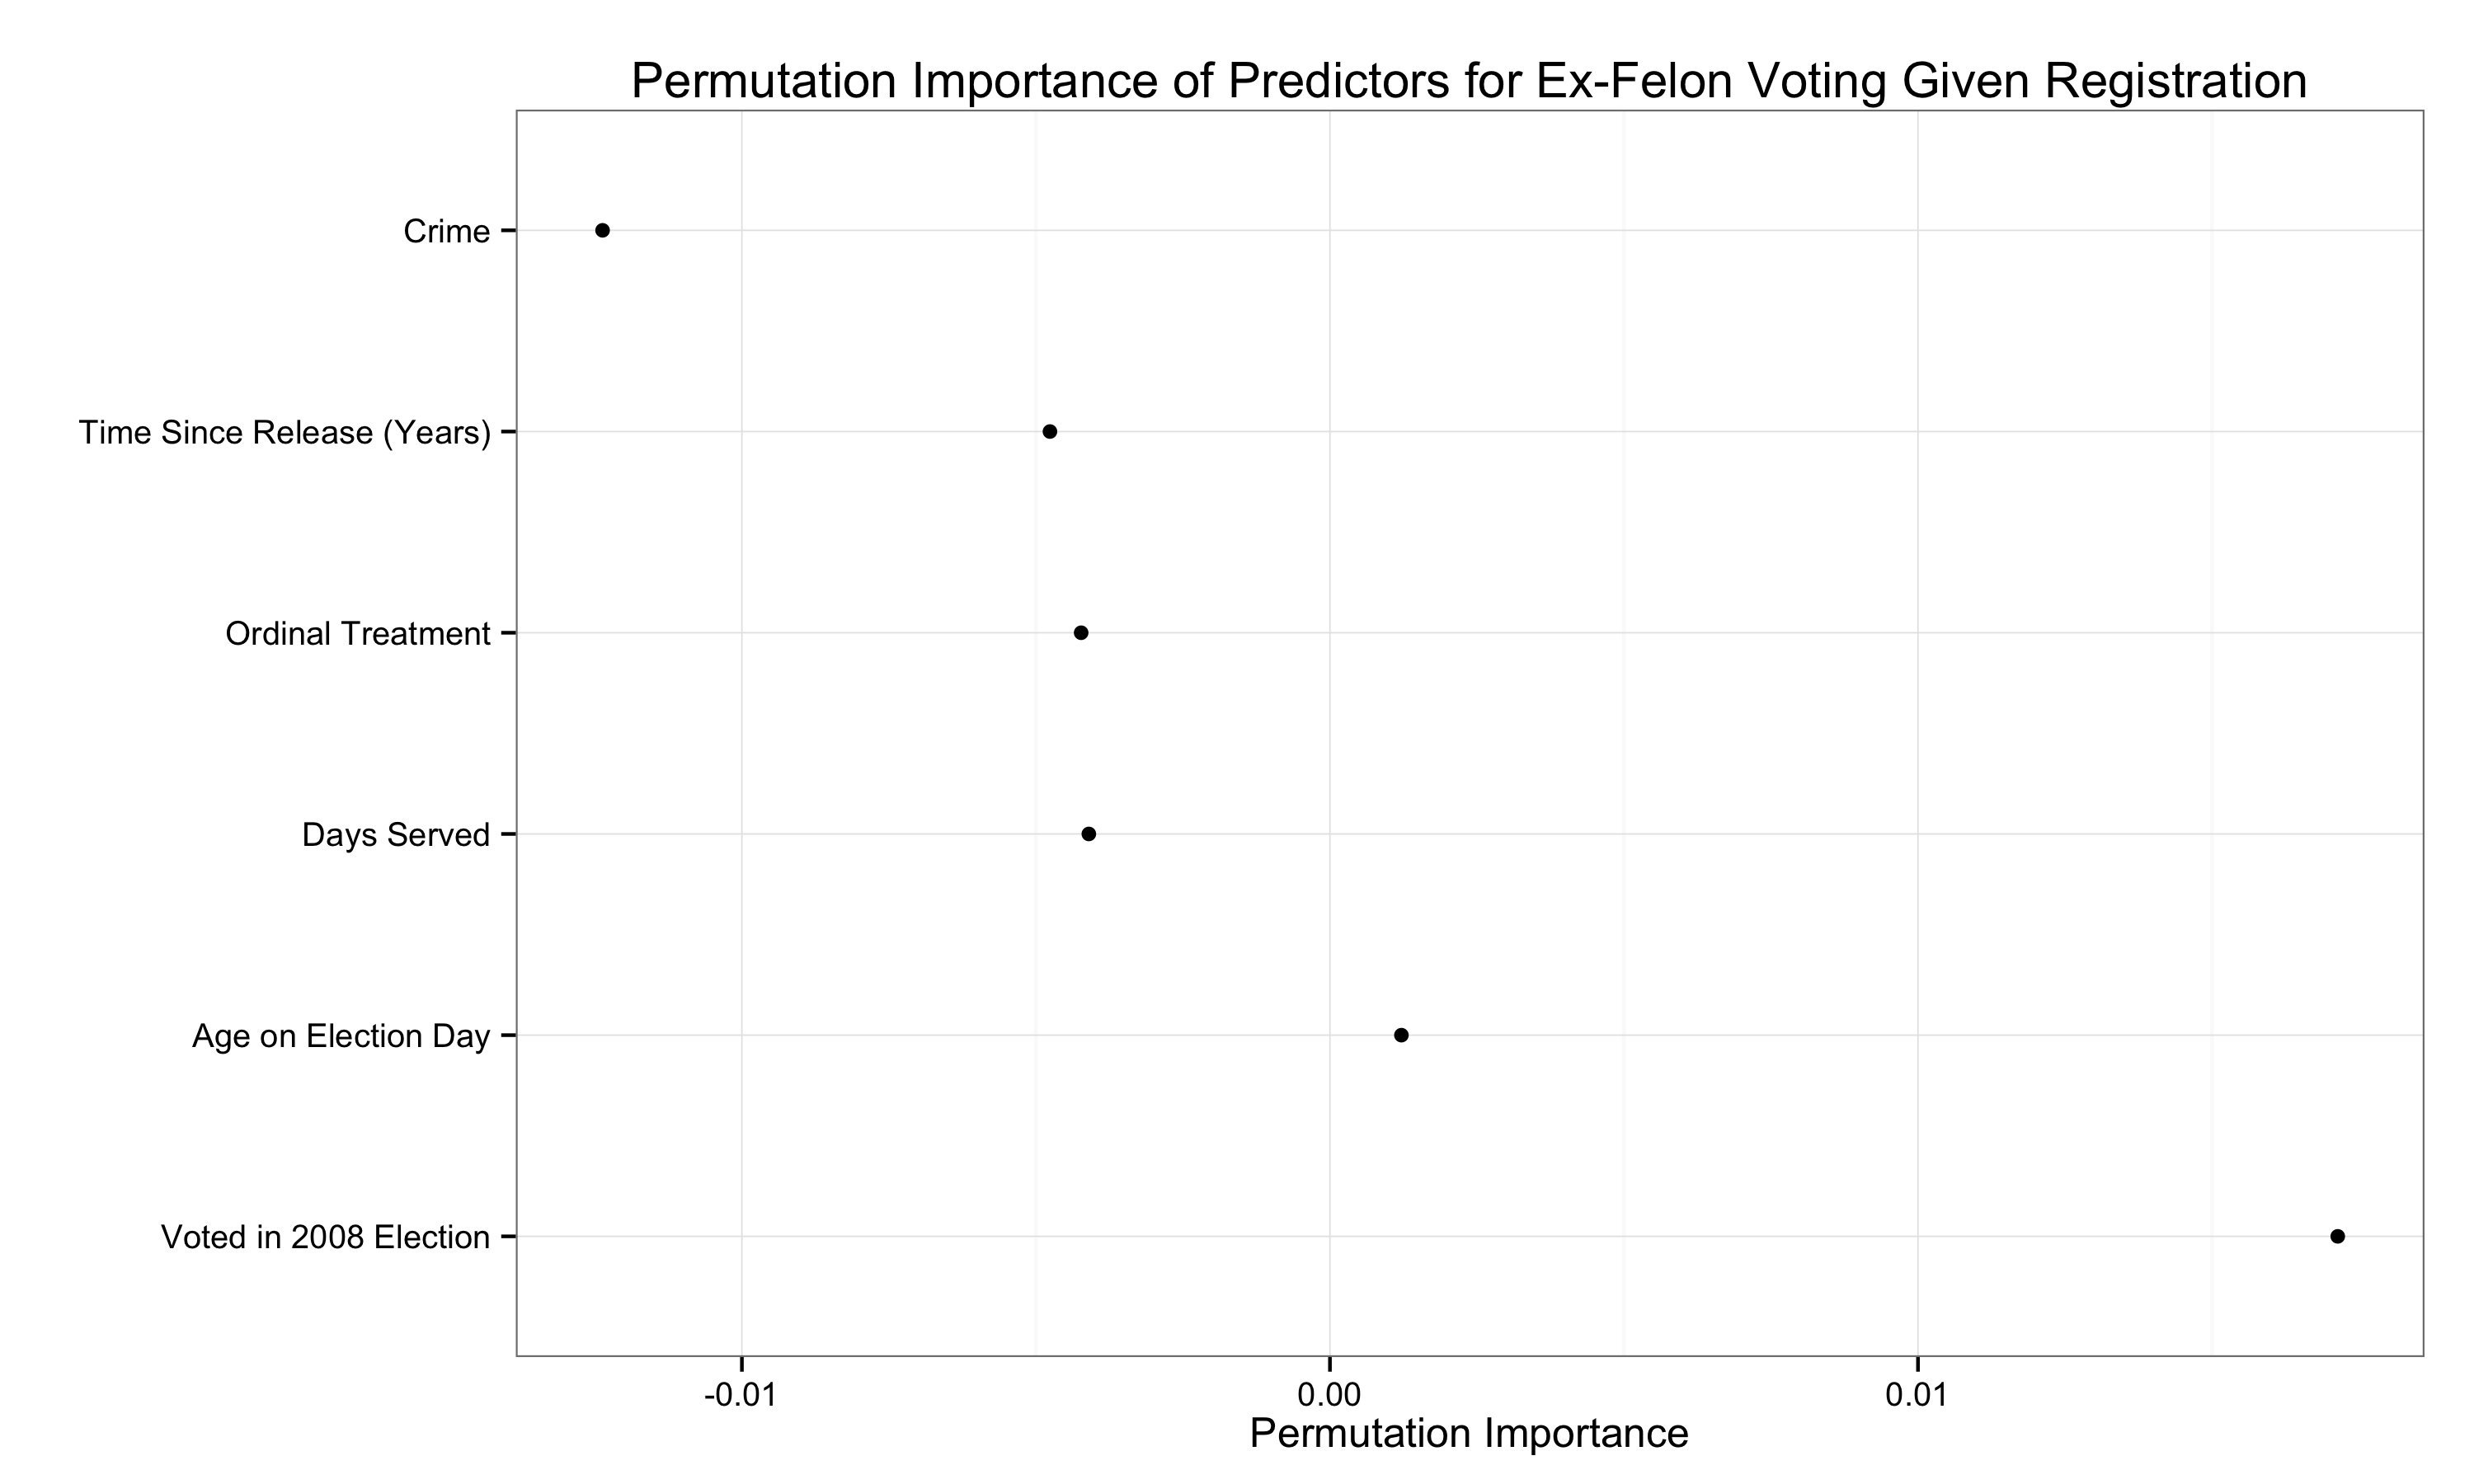
\includegraphics[width=\textwidth]{figures/imp_cond_vote.png}
                \caption{Permutation importance of predictors of vote conditional on registration for prisoners data.}
                \label{fig:imp_cond_vote}
        \end{subfigure}
        \caption{The marginal permutation importance of explanatory variables for the prediction of voter registration. The dots display the mean increase in classification error that results from randomly permuting the variable indicated. If the variable is important, permuting its values should systematically \textit{decrease} predictive performance (\textit{increasing} error), whereas an unimportant variable should produce no decrease, or a random decrease in error.}
        \label{fig:imp}
\end{figure}
